\chapter{Interfaz del Sistema}
\label{app-interfazdelsistema}

En el presente ap�ndice se presentan las principales interfaces del sistema implementadas para la Gesti�n de Consultas de �lgebra Relacional. \\

\begin{itemize}

\item \textbf{Login y Registro}: En la Figura \ref{fig:interfazloginyregistro} se presenta la interfaz del Login y el Registro de la aplicaci�n. Para logearse basta con ingresar el Rut y la Contrase�a, para Registrarse hay que ingresar el Rut del nuevo alumno, su contrase�a y una confirmaci�n de esta �ltima. \\ 

\begin{figure}[h!]
\centering
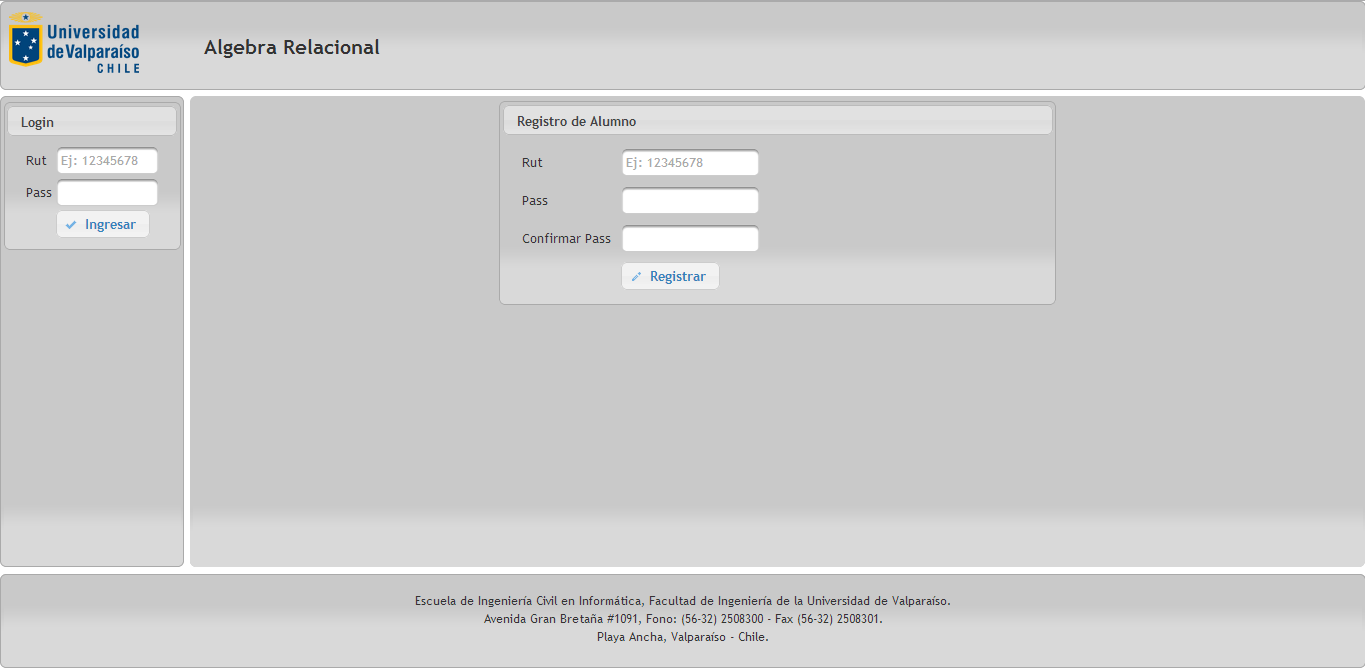
\includegraphics[width=15cm]{imagenes/captura_login.png}
\caption{Interfaz de Login y Registro.}
\label{fig:interfazloginyregistro}
\end{figure}

\newpage
\item \textbf{Crear Cuenta}: En la Figura \ref{fig:interfazcrearcuenta} se presenta la interfaz para la creaci�n de una Cuenta de Alumno. Para ello, se debe llenar cada uno de los formularios que aparecen, para finalmente confirmar el nuevo ingreso. \\

\begin{figure}[h!]
\centering
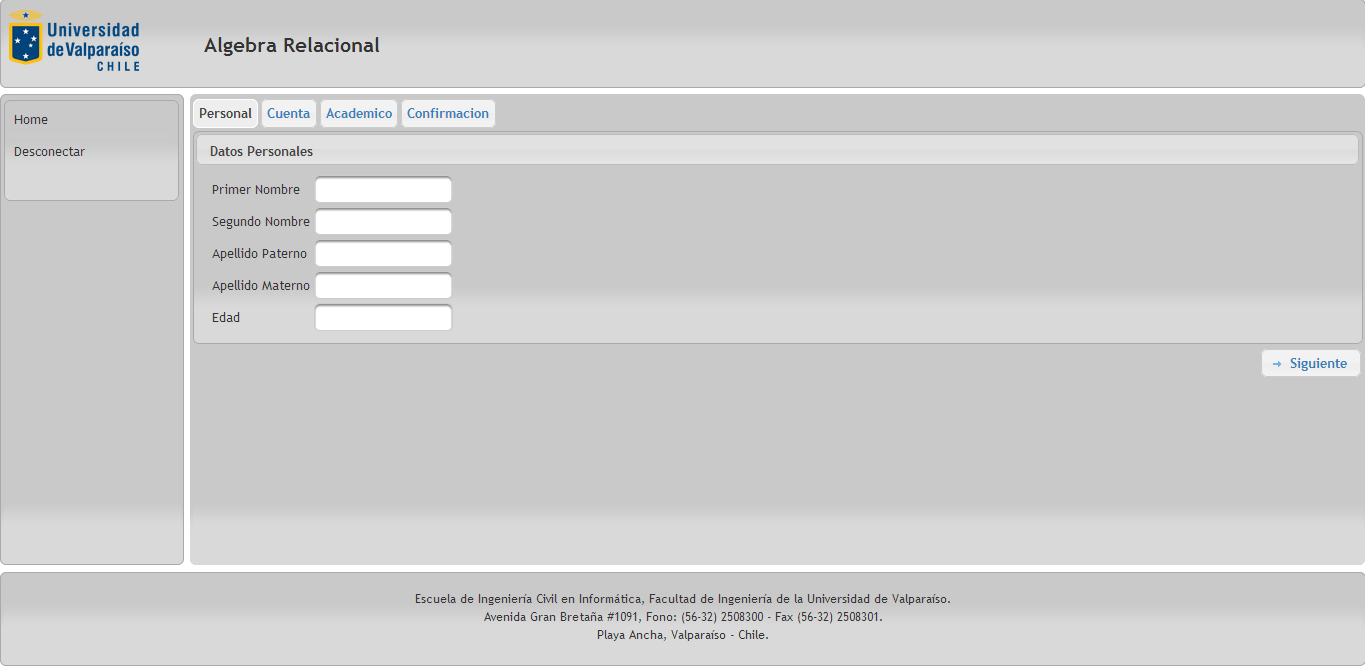
\includegraphics[width=15cm]{imagenes/captura_crear_cuenta.png}
\caption{Interfaz Crear Cuenta.}
\label{fig:interfazcrearcuenta}
\end{figure}

\newpage
\item \textbf{Eliminar Cuenta}: En la Figura \ref{fig:interfazeliminarcuenta} se presenta la interfaz para Eliminar Cuentas de Alumnos. Haciendo b�squeda utilizando cualquiera de los filtros, se selecciona el alumno a eliminar, para finalmente confirmar. \\

\begin{figure}[h!]
\centering
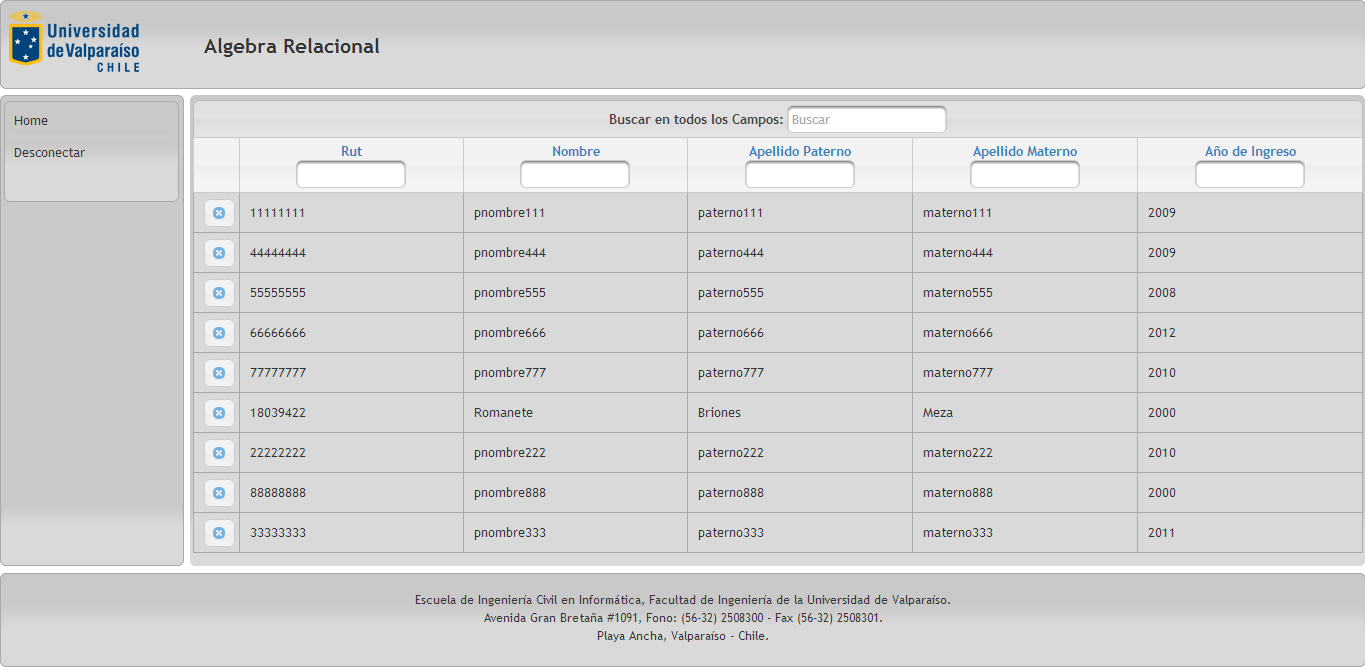
\includegraphics[width=15cm]{imagenes/captura_eliminar_cuenta.png}
\caption{Interfaz Eliminar Cuenta.}
\label{fig:interfazeliminarcuenta}
\end{figure}

\newpage
\item \textbf{Modificar Cuenta}: En la Figura \ref{fig:interfazmodificarcuenta} se presenta la interfaz para Modificar Cuentas de Alumnos. Haciendo b�squeda utilizando cualquiera de los filtros, se selecciona el alumno a modificar, para finalmente confirmar. \\

\begin{figure}[h!]
\centering
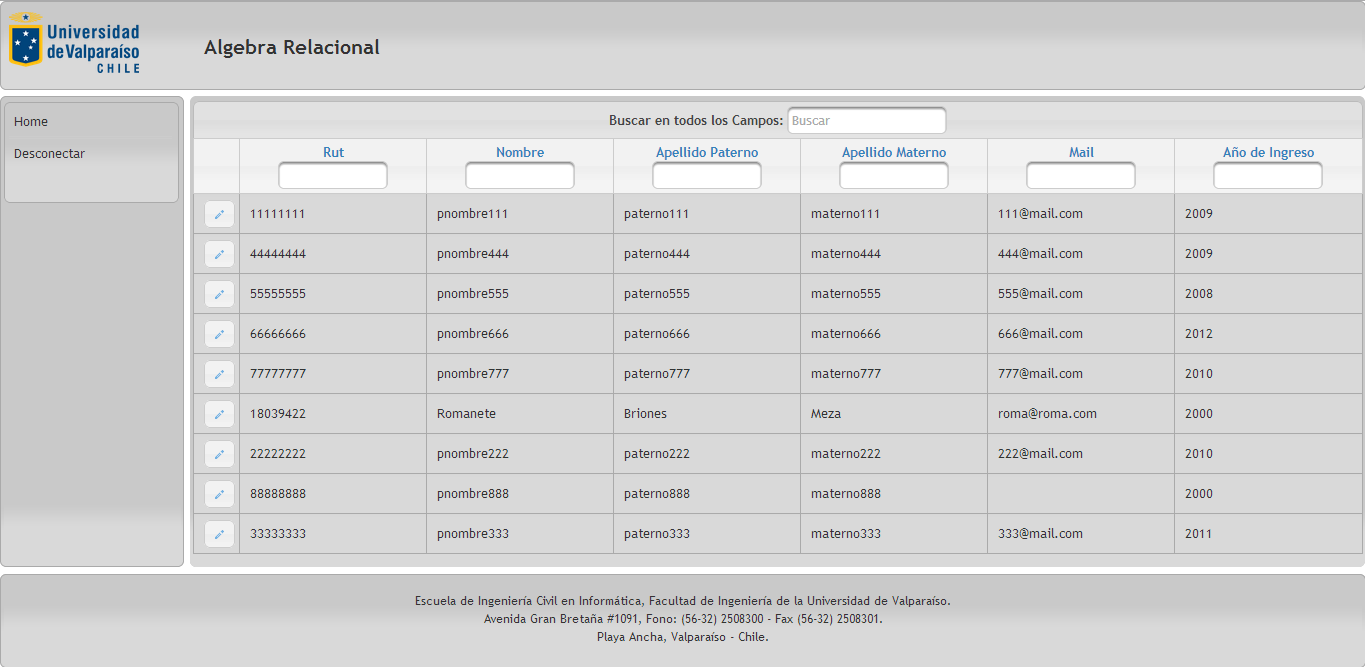
\includegraphics[width=15cm]{imagenes/captura_modificar_cuenta.png}
\caption{Interfaz Modificar Cuenta.}
\label{fig:interfazmodificarcuenta}
\end{figure}

\newpage
\item \textbf{Cargar Base de Datos}: En la Figura \ref{fig:interfazcargarbd} se presenta la interfaz para Cargar Bases de Datos. Haciendo b�squeda utilizando cualquiera de los filtros, se selecciona la base de datos a cargar, para finalmente confirmar. \\

\begin{figure}[h!]
\centering
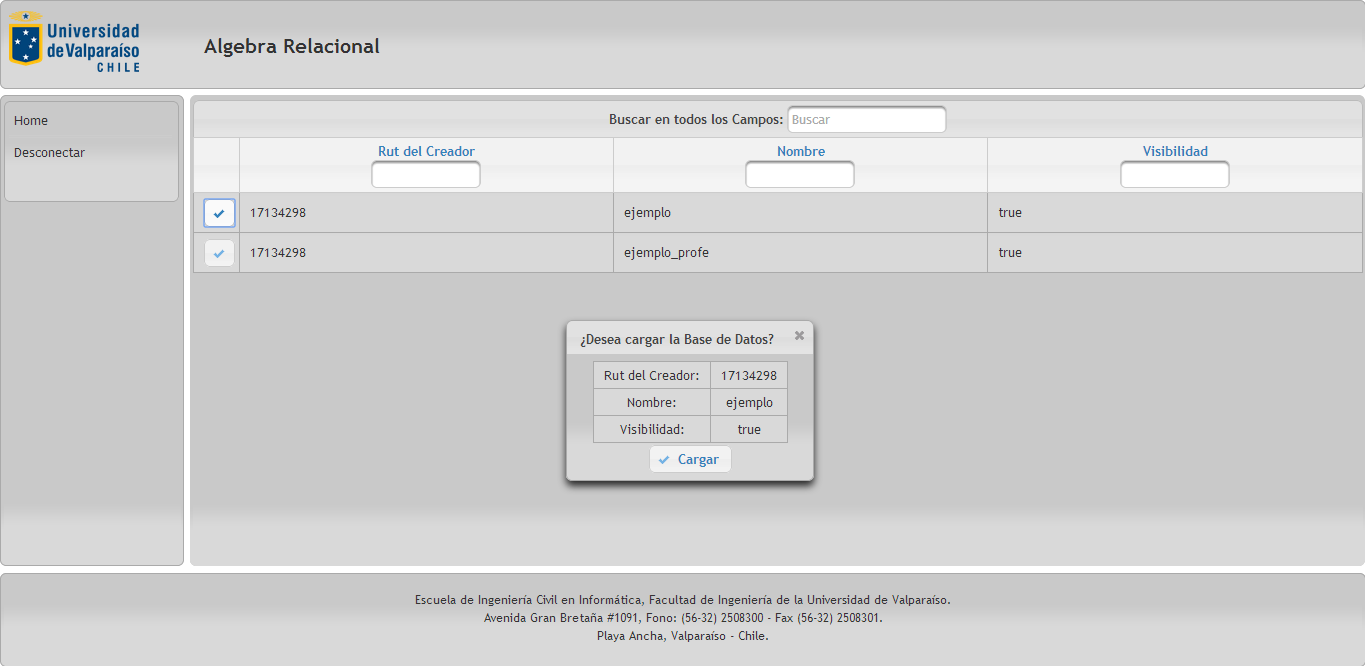
\includegraphics[width=15cm]{imagenes/captura_cargar_bd.png}
\caption{Interfaz Cargar Base de Datos.}
\label{fig:interfazcargarbd}
\end{figure}

\newpage
\item \textbf{Hacer Consulta}: En la Figura \ref{fig:interfazhacerconsulta} se presenta la interfaz para Hacer Consultas a una base de datos. Seleccionando cualquiera de los botones de ayuda para las consultas o ingresando v�a teclado la consulta de �lgebra Relacional, el sistema retorna el resultado de ella. \\

\begin{figure}[h!]
\centering
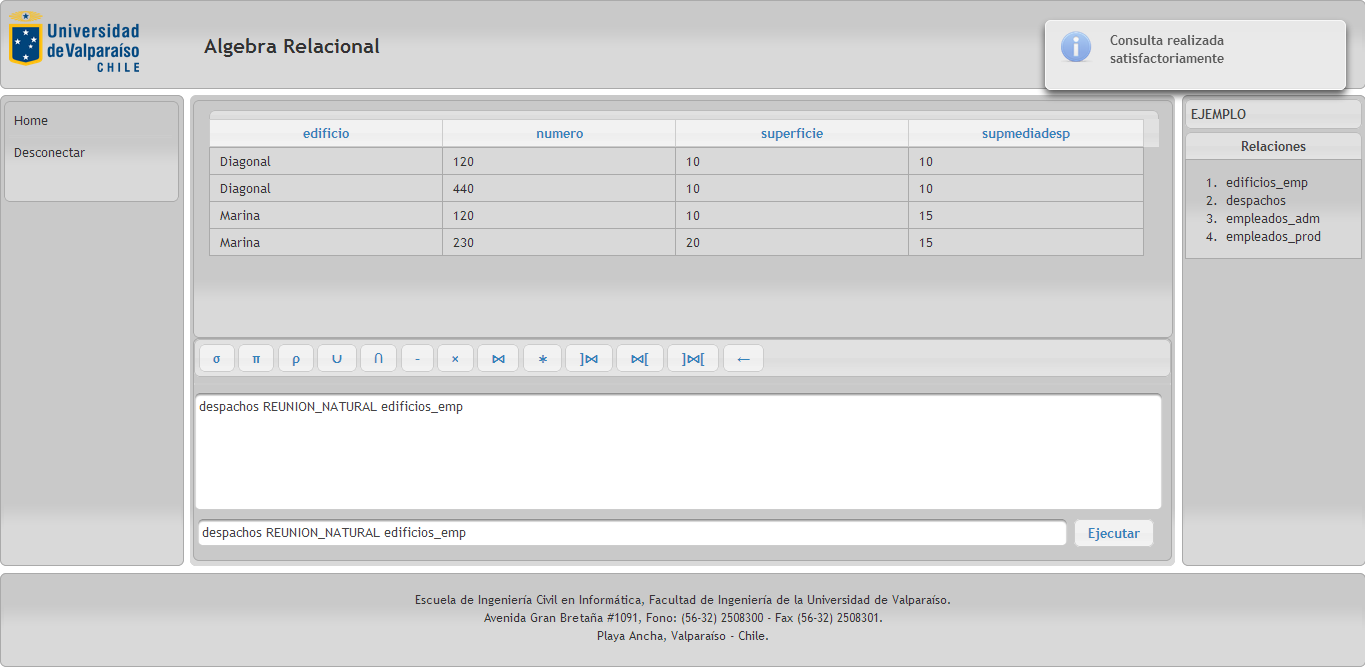
\includegraphics[width=15cm]{imagenes/captura_hacer_consulta.png}
\caption{Interfaz Hacer Consultas.}
\label{fig:interfazhacerconsulta}
\end{figure}

\newpage
\item \textbf{Gestionar Ejercicios}: En la Figura \ref{fig:interfazgestionarejercicios} se presenta la interfaz para la Gesti�n de Ejercicios. Aqu� se puede seleccionar la cantidad de ejercicios que tendr� la base de datos, y por cada uno de ellos se debe especificar la pregunta, la relaci�n resultante y las consultas para resolver ese ejercicio. Adem�s, es posible realizar consultas para verificar la correctitud de �stas. \\ 

\begin{figure}[h!]
\centering
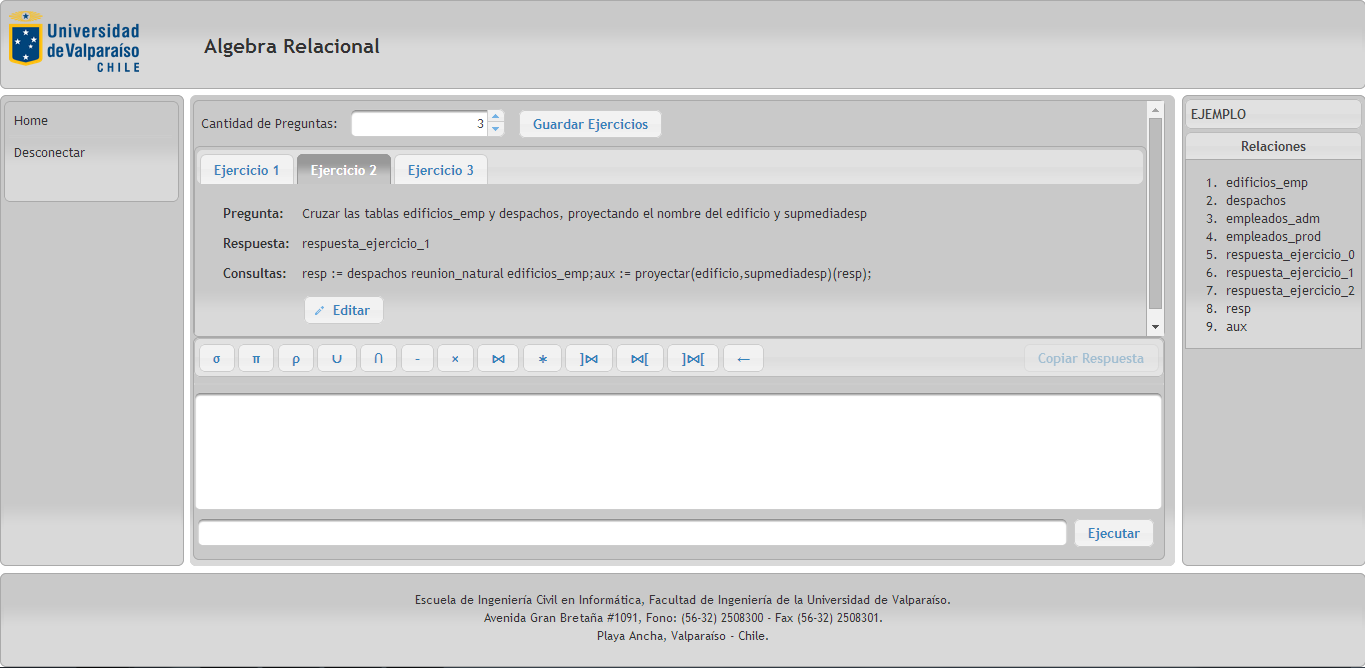
\includegraphics[width=15cm]{imagenes/captura_gestionar_ejercicios.png}
\caption{Interfaz Gestionar Ejercicios.}
\label{fig:interfazgestionarejercicios}
\end{figure}

\newpage
\item \textbf{Responder Ejercicios}: En la Figura \ref{fig:interfazresponderejercicios} se presenta la interfaz para Responder Ejercicios. Aqu� se puede seleccionar el ejercicio a responder y su respectiva respuesta. Adem�s, es posible realizar consultas para verificar la correctitud de �stas. Finalmente se env�a el formulario para obtener la calificaci�n. \\ 

\begin{figure}[h!]
\centering
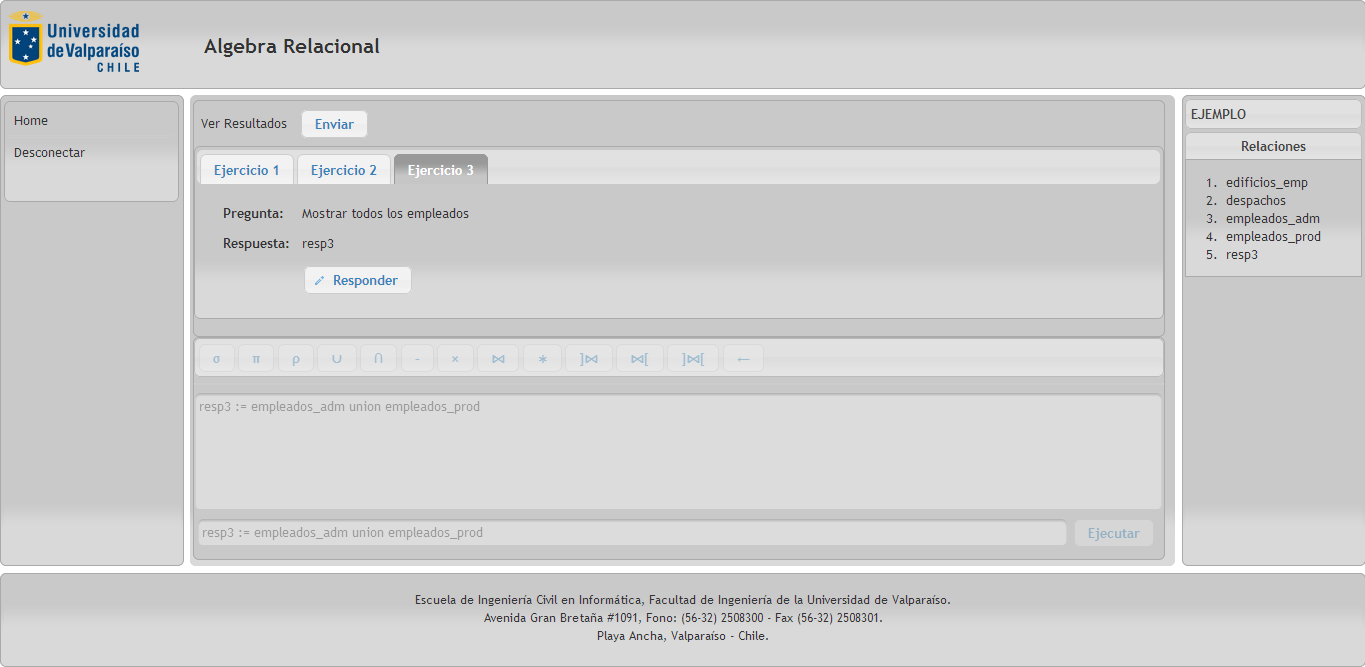
\includegraphics[width=15cm]{imagenes/captura_responder_ejercicio.png}
\caption{Interfaz Responder Ejercicios.}
\label{fig:interfazresponderejercicios}
\end{figure}

\newpage
\item \textbf{Obtener Calificaci�n}: En la Figura \ref{fig:interfazobtenercalificacion} se presenta la interfaz para la Obtenci�n de Calificaci�n, luego de responder un serie de Ejercicios. En esta interfaz se muestran el resultado de los ejercicios y la respuesta esperada de ellos. \\

\begin{figure}[h!]
\centering
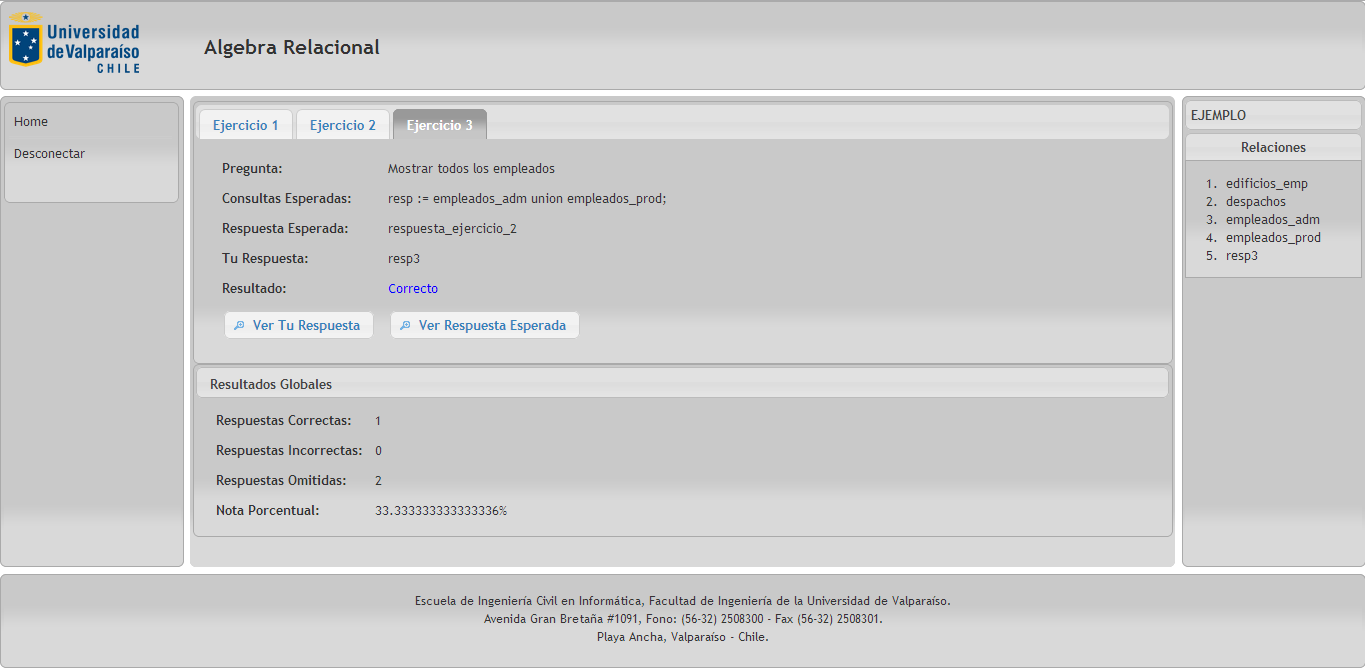
\includegraphics[width=15cm]{imagenes/captura_obtener_calificacion.png}
\caption{Interfaz Obtener Calificaci�n.}
\label{fig:interfazobtenercalificacion}
\end{figure}

\newpage
\item \textbf{Ver Estad�sticas}: En la Figura \ref{fig:interfazverestadisticas} se presenta la interfaz para la Visualizaci�n de Estad�sticas de los Ejercicios. En esta interfaz se observan los valores estad�sticos principales de todos los ejercicios de la base de datos cargada. Adem�s, consta con un gr�fico que muestra la cantidad de respuestas, intentos y errores de cada ejercicio. \\

\begin{figure}[h!]
\centering
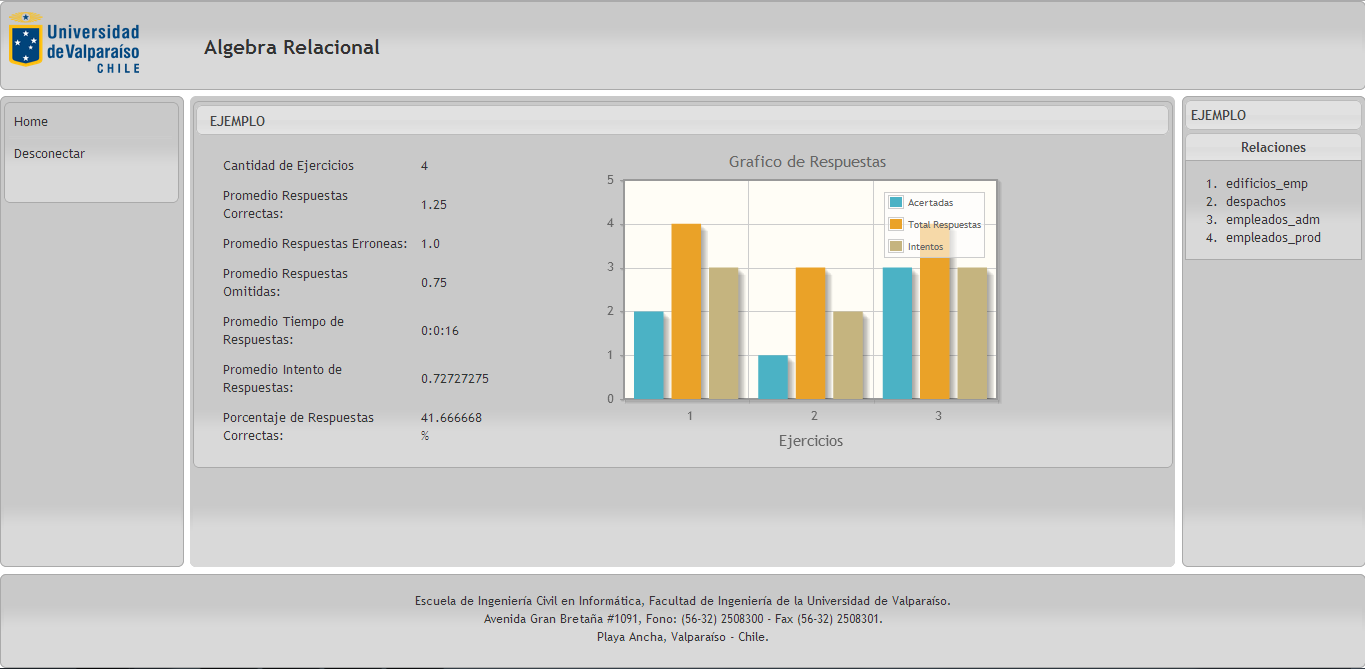
\includegraphics[width=15cm]{imagenes/captura_ver_estadisticas.png}
\caption{Interfaz Ver Estad�sticas}
\label{fig:interfazverestadisticas}
\end{figure}

\end{itemize}
